\section{失败诊断与恢复}
\label{chapter:05}

% block-id: auto.05.p1
\hypertarget{auto.05.p1}{}
失败诊断案例保留了一次实际单位换算 API 错误及其修复。原 MCP 调用的传输返回并不能单独代表业务执行成功：工具可能以普通字符串返回错误，而协议层 isError 仍为 false。诊断需要检查实际返回内容、异常上下文和预期结果结构，随后修正 API 调用，并在新运行中核对成功响应及后续求解产物。

% block-id: auto.05.p2
\hypertarget{auto.05.p2}{}
该修复保持原物理参数和约束。失败调用、修订后的调用与关联 Maxwell 结果构成对照，使读者能够识别修复发生在接口层。协议报告据此说明工具是否完成预期操作，物理报告则继续负责端口和功率验收；二者通过运行身份关联。

% block-id: auto.05.p3
\hypertarget{auto.05.p3}{}
A–φ 案例展示另一类诊断。执行器读取已有场、势和导数诊断，记录 completed 执行状态，同时保留 failed\_retained\_phi\_gauge 物理状态。采样参数和显示参数的修改只改变保存场的观察方式。原场输入、采样位置、诊断公式与验收门槛共同决定解释依据，后续修订需要回到势与规范条件的数值实现。\cite{FEMDOC}

% block-id: auto.05.figure
\hypertarget{auto.05.figure}{}
\begin{figure}[!htbp]
\centering
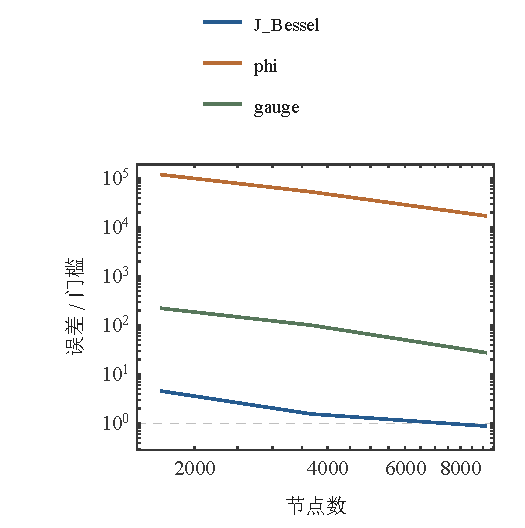
\includegraphics[width=\linewidth,height=.72\textheight,keepaspectratio]{../../assets/zh-CN/aphi_gates.pdf}
\caption{A–φ 圆柱校准指标。 三档网格与各指标门槛分别展示。 圆柱三档含 1683、3672、9108 节点。误差以各自验收门槛归一化，水平线标出单位比值。}
\label{fig:aphi_gates}
\end{figure}

% block-id: auto.05.p4
\hypertarget{auto.05.p4}{}
Wolfram 工具记录还包含前端工作完成后的进程清理：保存回执已确认，所属辅助进程最终退出码为 137，清理原因单独记录。分析这类运行时，需要同时读取完成回执、已保存产物和进程终止原因。单个退出码无法完整表达跨前端与内核的工作状态。

% block-id: auto.05.p5
\hypertarget{auto.05.p5}{}
归档的 rc.2 六类案例共同覆盖校准与 Notebook、原生建模求解、跨求解器比较、源码扩展、接口修复及数值失败解释。其共同产物是可定位的输入、源码、调用、结果和验收说明。接手者可以选择具体失败层重现问题，并以新的运行身份继续研究。
